\begin{figure}[ht]
\begin{center}
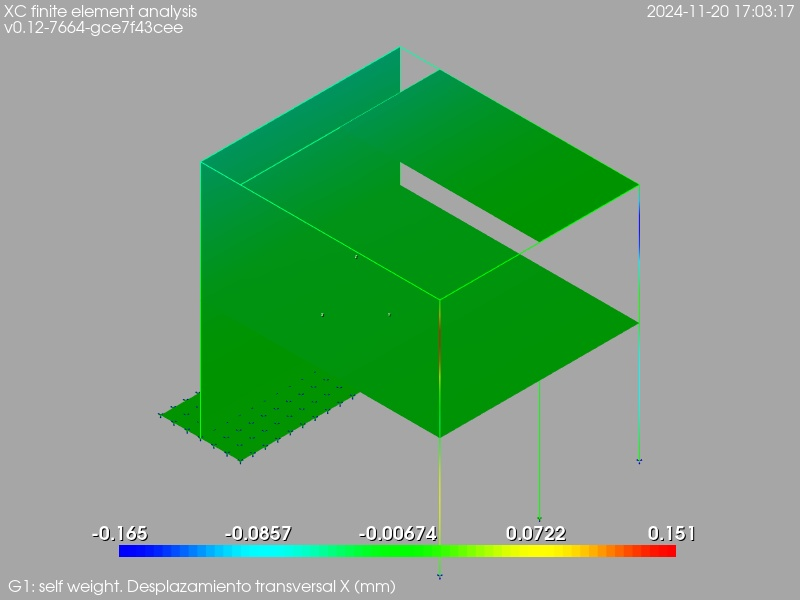
\includegraphics[width=\linewidth]{results/graphics/resSimplLC/GselfWeightuX.png}
\caption{ G1: self weight. Desplazamiento transversal X (mm)}
\label{GselfWeightuX}
\end{center}
\end{figure}
\begin{figure}[ht]
\begin{center}
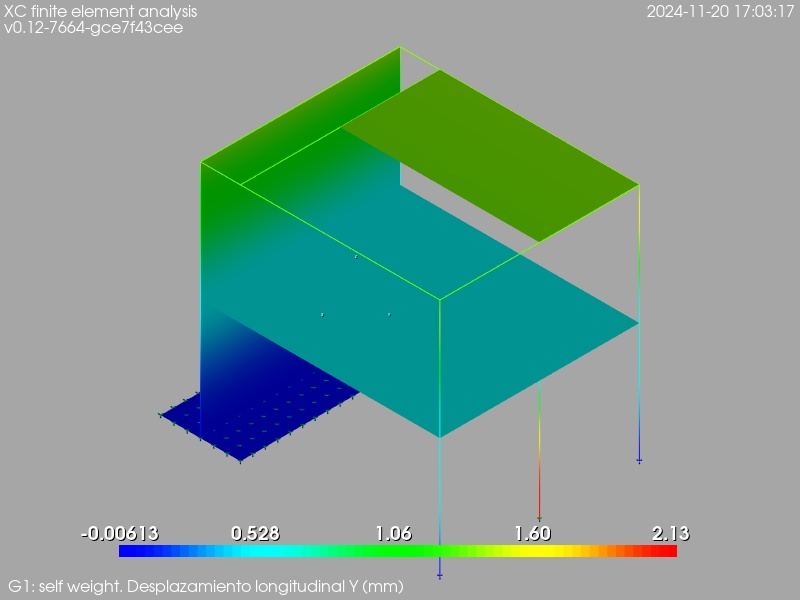
\includegraphics[width=\linewidth]{results/graphics/resSimplLC/GselfWeightuY.png}
\caption{ G1: self weight. Desplazamiento longitudinal Y (mm)}
\label{GselfWeightuY}
\end{center}
\end{figure}
\begin{figure}[ht]
\begin{center}
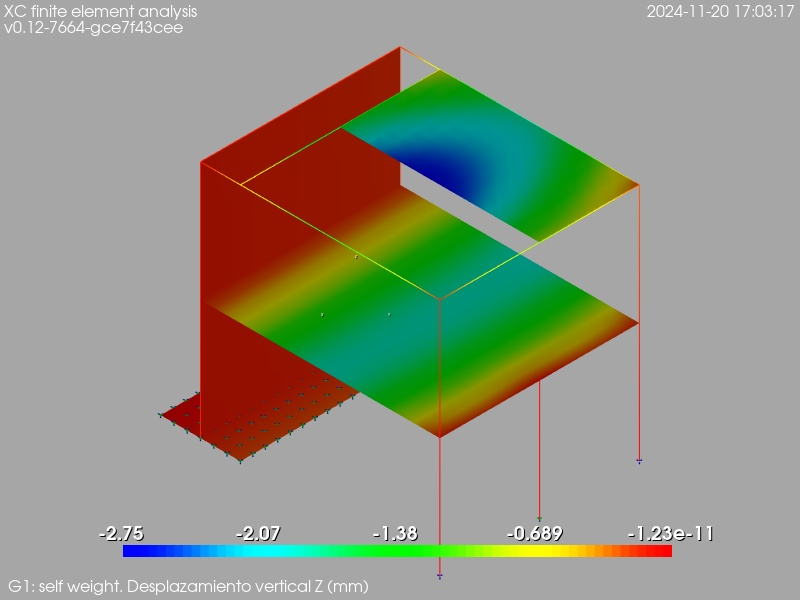
\includegraphics[width=\linewidth]{results/graphics/resSimplLC/GselfWeightuZ.png}
\caption{ G1: self weight. Desplazamiento vertical Z (mm)}
\label{GselfWeightuZ}
\end{center}
\end{figure}
\begin{figure}[ht]
\begin{center}
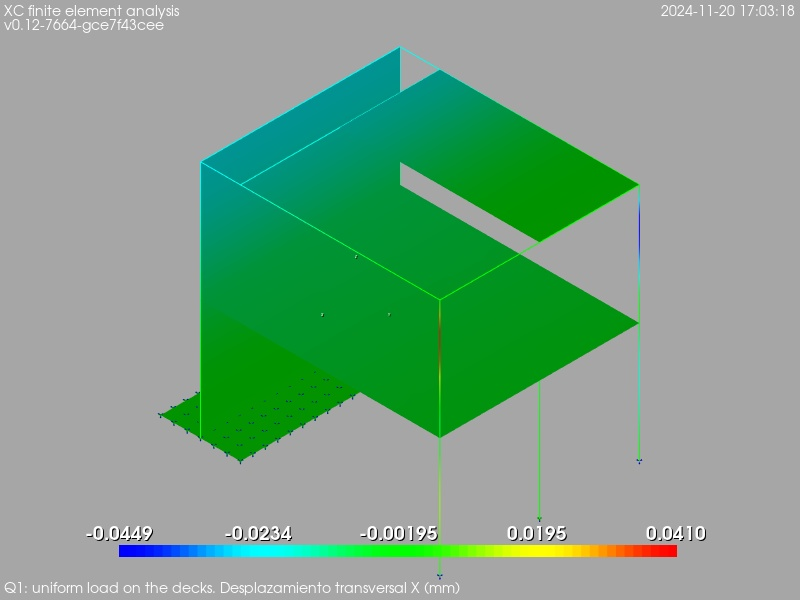
\includegraphics[width=\linewidth]{results/graphics/resSimplLC/QdecksuX.png}
\caption{Q1: uniform load on the decks. Desplazamiento transversal X (mm)}
\label{QdecksuX}
\end{center}
\end{figure}
\begin{figure}[ht]
\begin{center}
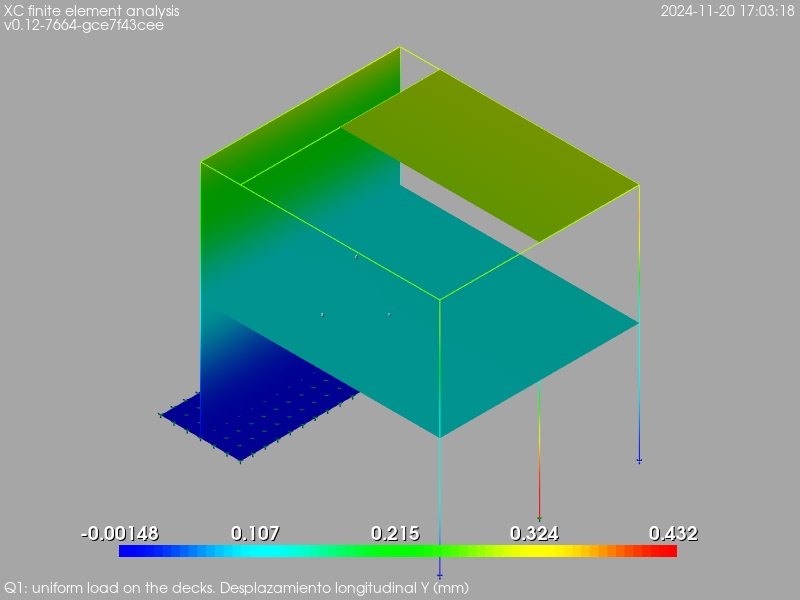
\includegraphics[width=\linewidth]{results/graphics/resSimplLC/QdecksuY.png}
\caption{Q1: uniform load on the decks. Desplazamiento longitudinal Y (mm)}
\label{QdecksuY}
\end{center}
\end{figure}
\begin{figure}[ht]
\begin{center}
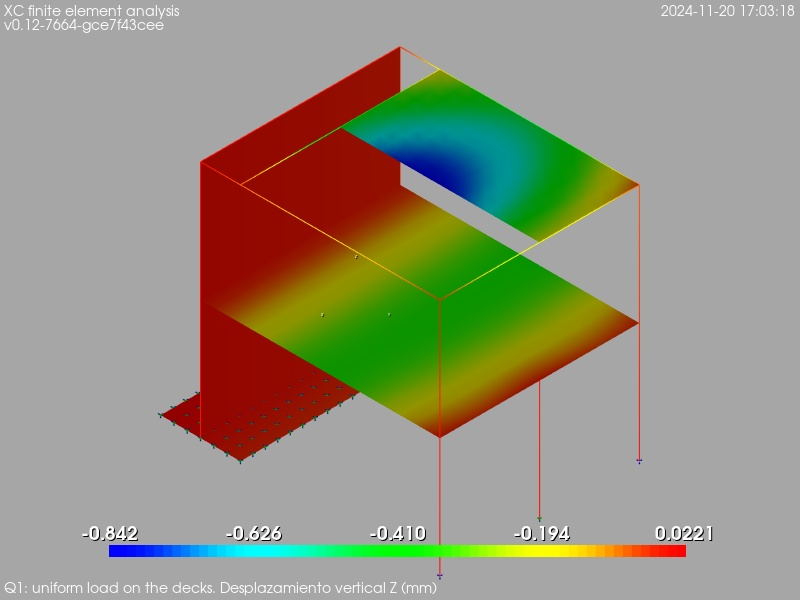
\includegraphics[width=\linewidth]{results/graphics/resSimplLC/QdecksuZ.png}
\caption{Q1: uniform load on the decks. Desplazamiento vertical Z (mm)}
\label{QdecksuZ}
\end{center}
\end{figure}
\begin{figure}[ht]
\begin{center}
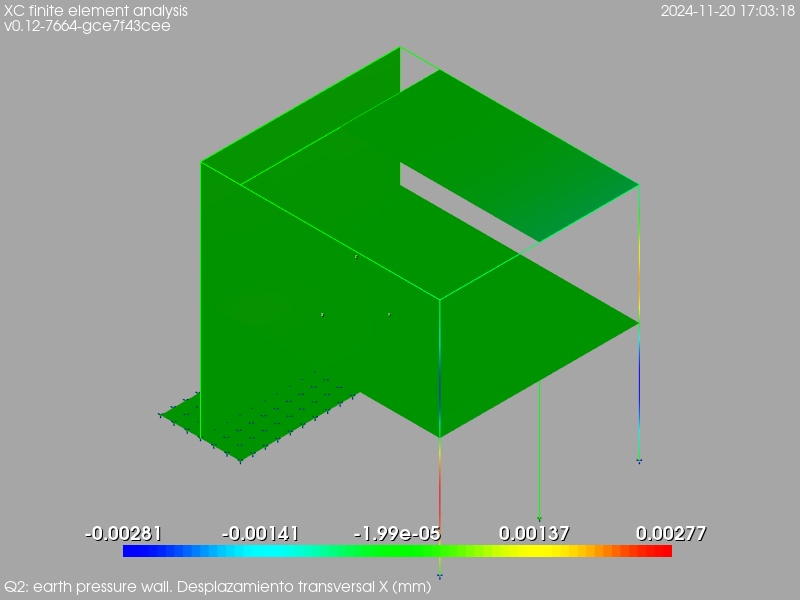
\includegraphics[width=\linewidth]{results/graphics/resSimplLC/QearthPressWalluX.png}
\caption{Q2: earth pressure wall. Desplazamiento transversal X (mm)}
\label{QearthPressWalluX}
\end{center}
\end{figure}
\begin{figure}[ht]
\begin{center}
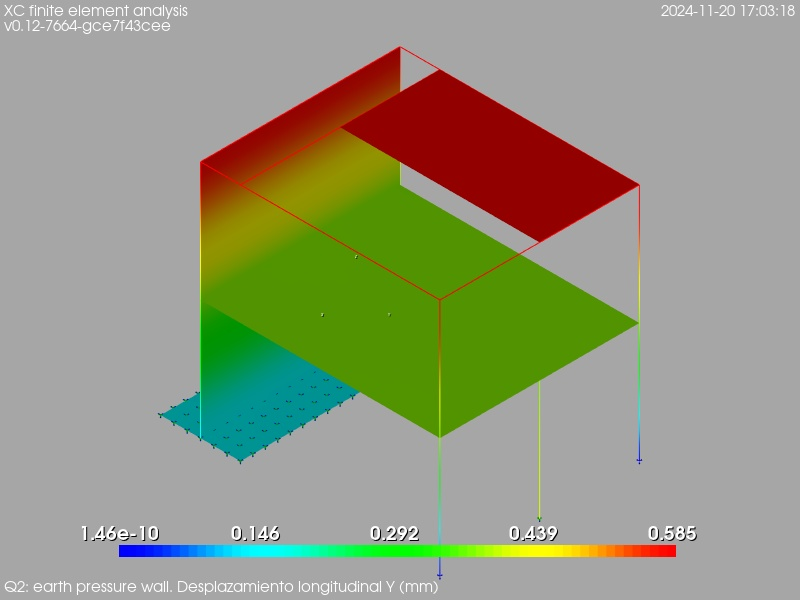
\includegraphics[width=\linewidth]{results/graphics/resSimplLC/QearthPressWalluY.png}
\caption{Q2: earth pressure wall. Desplazamiento longitudinal Y (mm)}
\label{QearthPressWalluY}
\end{center}
\end{figure}
\begin{figure}[ht]
\begin{center}
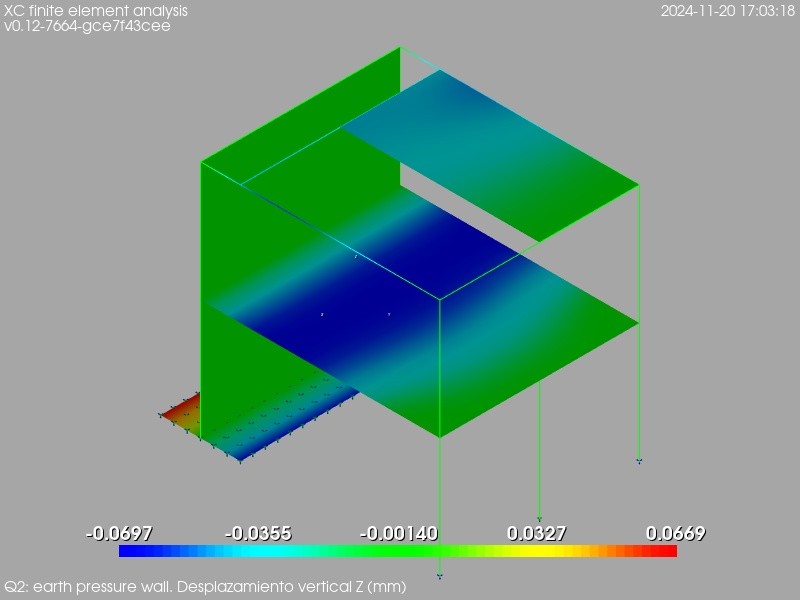
\includegraphics[width=\linewidth]{results/graphics/resSimplLC/QearthPressWalluZ.png}
\caption{Q2: earth pressure wall. Desplazamiento vertical Z (mm)}
\label{QearthPressWalluZ}
\end{center}
\end{figure}
\begin{figure}[ht]
\begin{center}
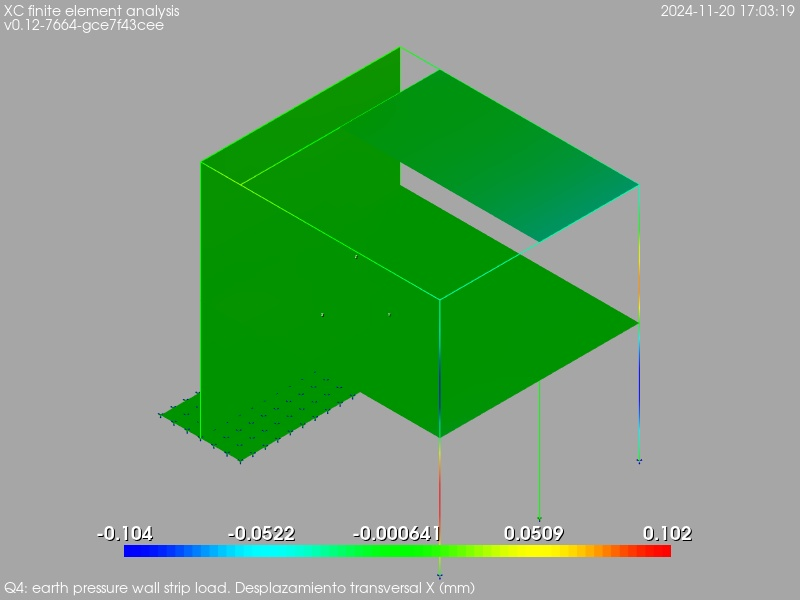
\includegraphics[width=\linewidth]{results/graphics/resSimplLC/QearthPWallStrLuX.png}
\caption{Q4: earth pressure wall strip load. Desplazamiento transversal X (mm)}
\label{QearthPWallStrLuX}
\end{center}
\end{figure}
\begin{figure}[ht]
\begin{center}
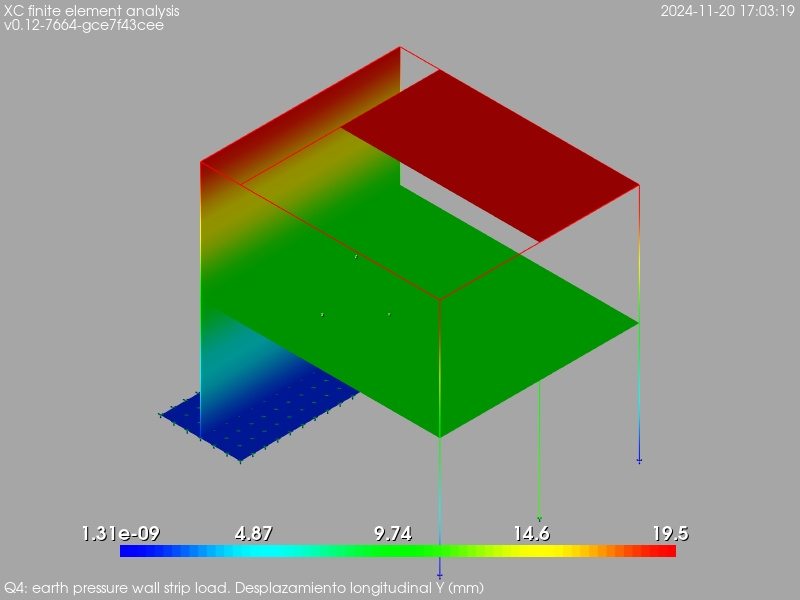
\includegraphics[width=\linewidth]{results/graphics/resSimplLC/QearthPWallStrLuY.png}
\caption{Q4: earth pressure wall strip load. Desplazamiento longitudinal Y (mm)}
\label{QearthPWallStrLuY}
\end{center}
\end{figure}
\begin{figure}[ht]
\begin{center}
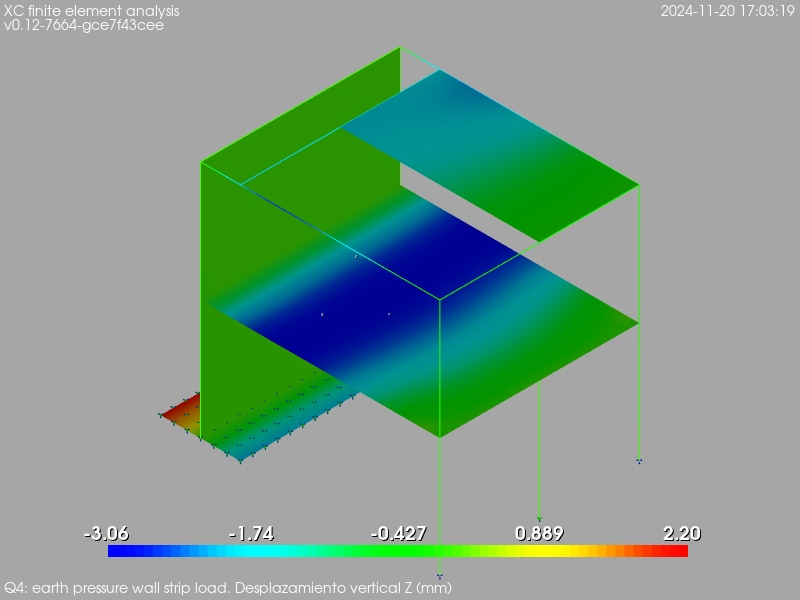
\includegraphics[width=\linewidth]{results/graphics/resSimplLC/QearthPWallStrLuZ.png}
\caption{Q4: earth pressure wall strip load. Desplazamiento vertical Z (mm)}
\label{QearthPWallStrLuZ}
\end{center}
\end{figure}
\begin{figure}[ht]
\begin{center}
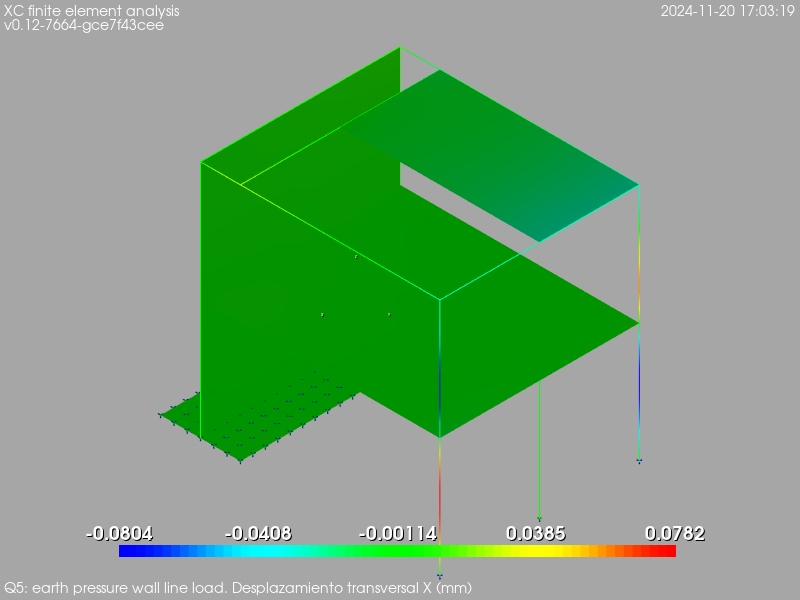
\includegraphics[width=\linewidth]{results/graphics/resSimplLC/QearthPWallLinLuX.png}
\caption{Q5: earth pressure wall line load. Desplazamiento transversal X (mm)}
\label{QearthPWallLinLuX}
\end{center}
\end{figure}
\begin{figure}[ht]
\begin{center}
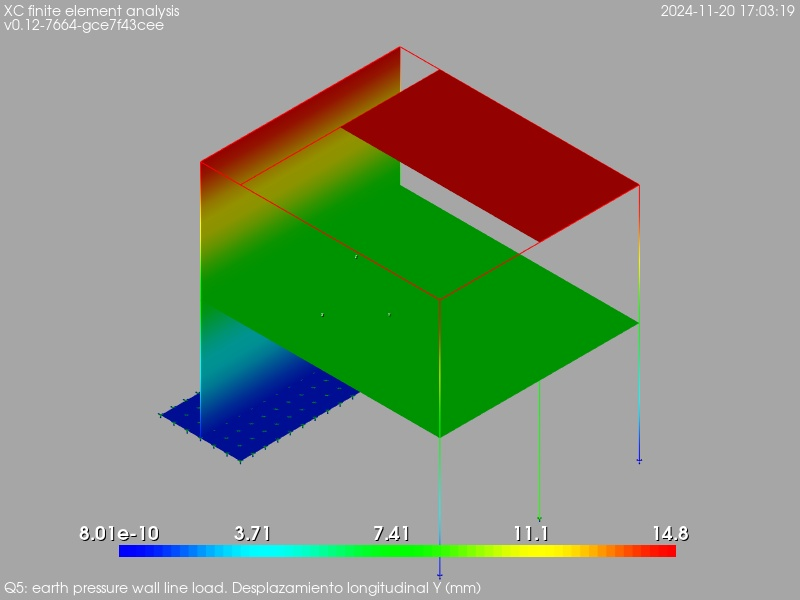
\includegraphics[width=\linewidth]{results/graphics/resSimplLC/QearthPWallLinLuY.png}
\caption{Q5: earth pressure wall line load. Desplazamiento longitudinal Y (mm)}
\label{QearthPWallLinLuY}
\end{center}
\end{figure}
\begin{figure}[ht]
\begin{center}
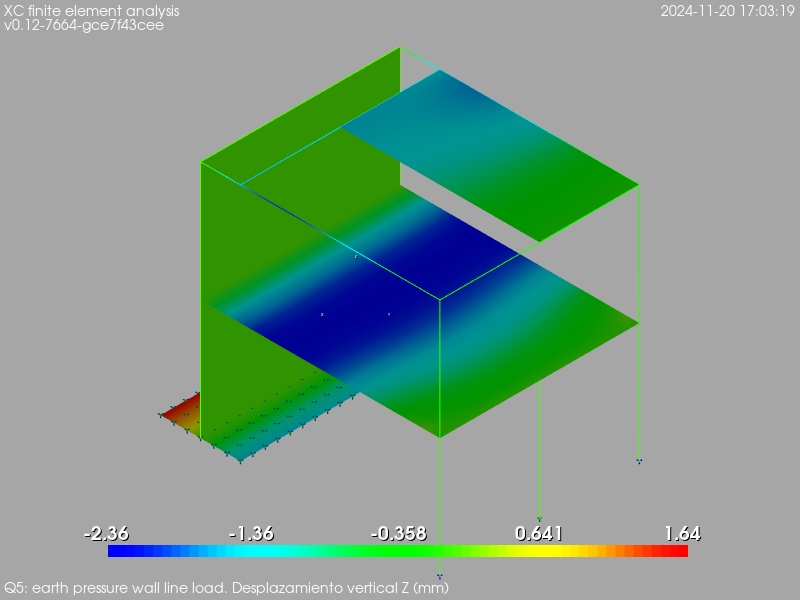
\includegraphics[width=\linewidth]{results/graphics/resSimplLC/QearthPWallLinLuZ.png}
\caption{Q5: earth pressure wall line load. Desplazamiento vertical Z (mm)}
\label{QearthPWallLinLuZ}
\end{center}
\end{figure}
\begin{figure}[ht]
\begin{center}
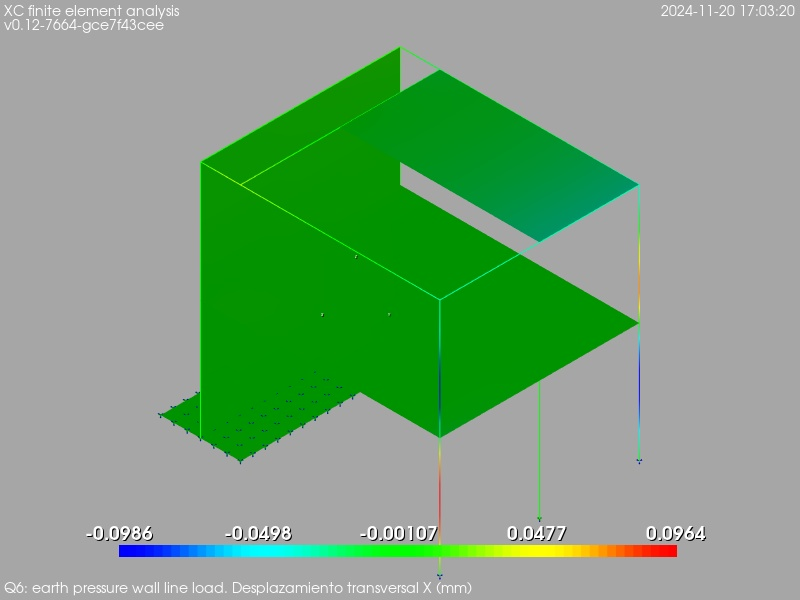
\includegraphics[width=\linewidth]{results/graphics/resSimplLC/QearthPWallHrzLuX.png}
\caption{Q6: earth pressure wall line load. Desplazamiento transversal X (mm)}
\label{QearthPWallHrzLuX}
\end{center}
\end{figure}
\begin{figure}[ht]
\begin{center}
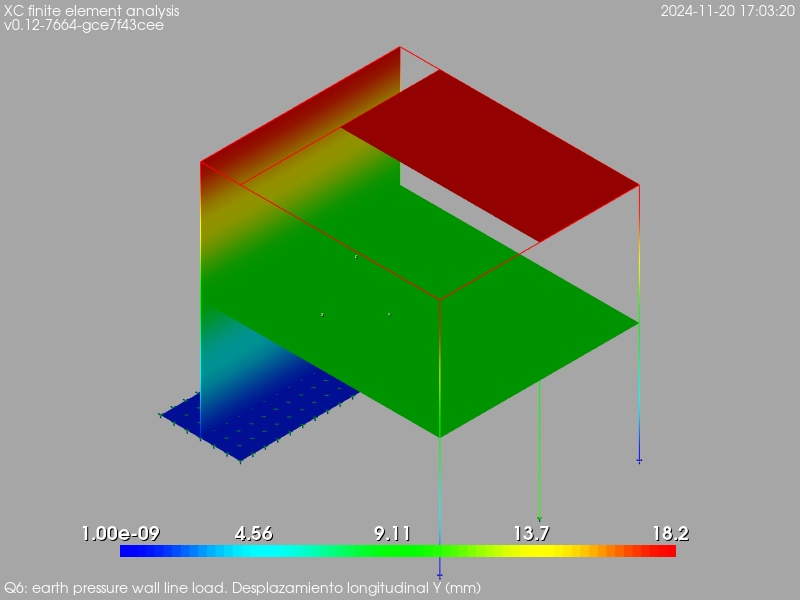
\includegraphics[width=\linewidth]{results/graphics/resSimplLC/QearthPWallHrzLuY.png}
\caption{Q6: earth pressure wall line load. Desplazamiento longitudinal Y (mm)}
\label{QearthPWallHrzLuY}
\end{center}
\end{figure}
\begin{figure}[ht]
\begin{center}
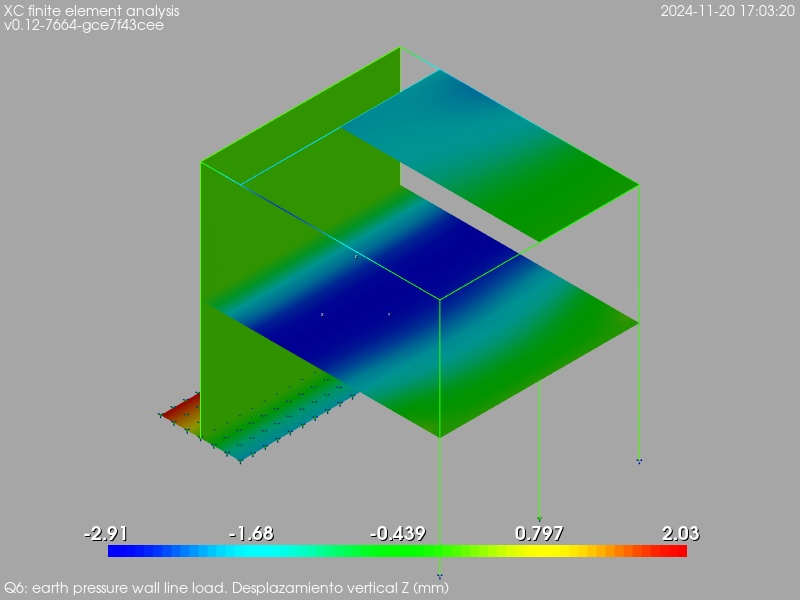
\includegraphics[width=\linewidth]{results/graphics/resSimplLC/QearthPWallHrzLuZ.png}
\caption{Q6: earth pressure wall line load. Desplazamiento vertical Z (mm)}
\label{QearthPWallHrzLuZ}
\end{center}
\end{figure}
\begin{figure}[ht]
\begin{center}
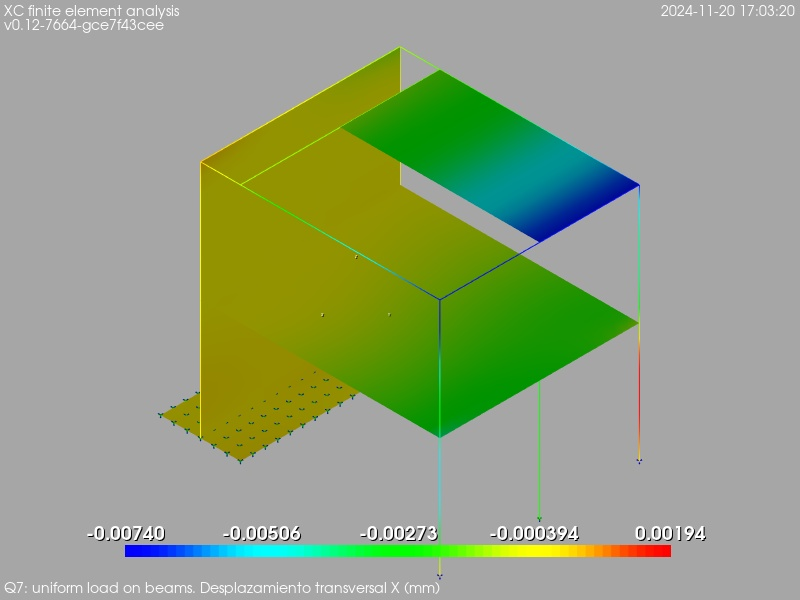
\includegraphics[width=\linewidth]{results/graphics/resSimplLC/qunifBeamsuX.png}
\caption{Q7: uniform load on beams. Desplazamiento transversal X (mm)}
\label{qunifBeamsuX}
\end{center}
\end{figure}
\begin{figure}[ht]
\begin{center}
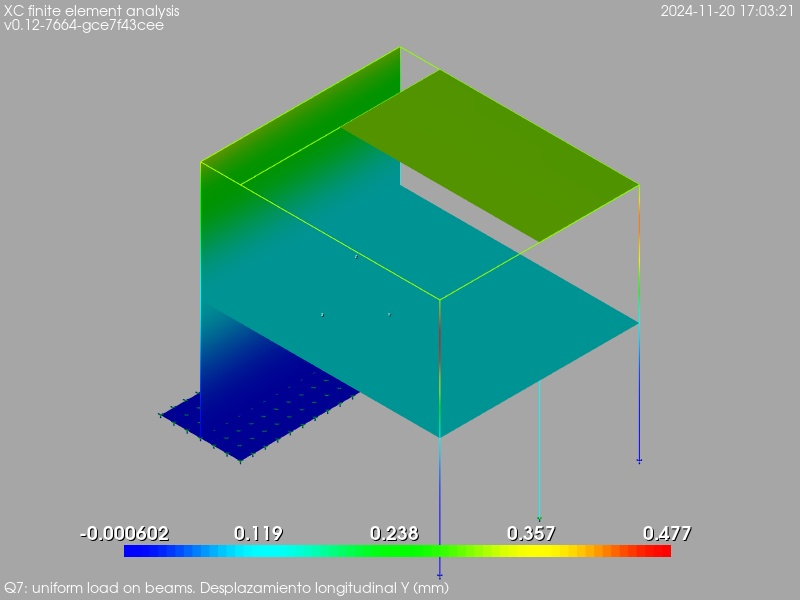
\includegraphics[width=\linewidth]{results/graphics/resSimplLC/qunifBeamsuY.png}
\caption{Q7: uniform load on beams. Desplazamiento longitudinal Y (mm)}
\label{qunifBeamsuY}
\end{center}
\end{figure}
\begin{figure}[ht]
\begin{center}
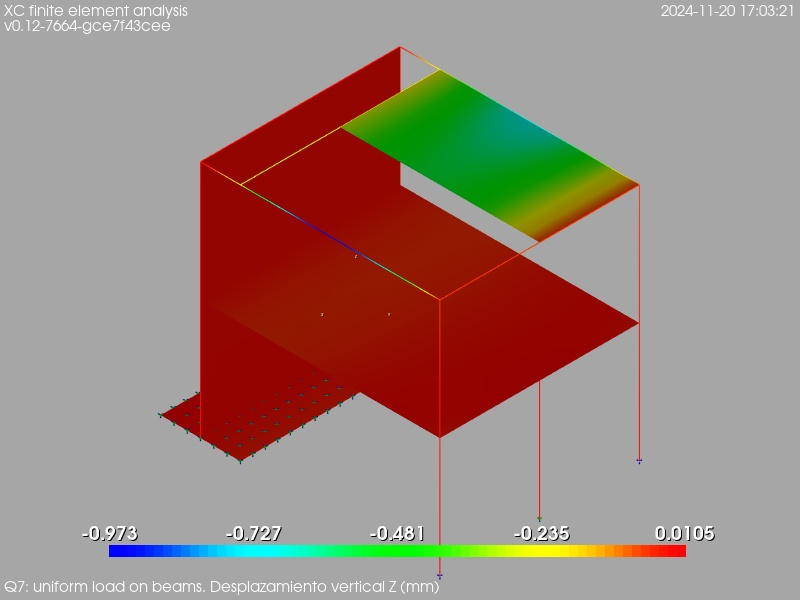
\includegraphics[width=\linewidth]{results/graphics/resSimplLC/qunifBeamsuZ.png}
\caption{Q7: uniform load on beams. Desplazamiento vertical Z (mm)}
\label{qunifBeamsuZ}
\end{center}
\end{figure}
\begin{figure}[ht]
\begin{center}
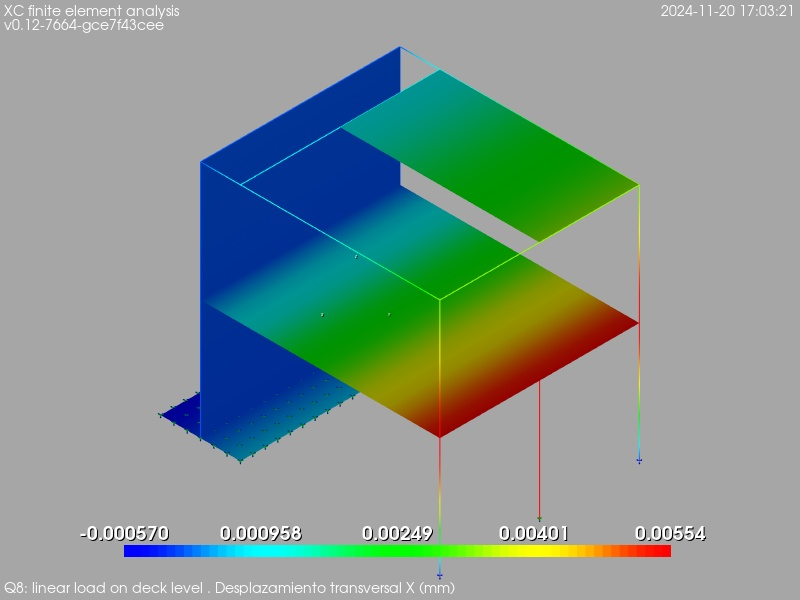
\includegraphics[width=\linewidth]{results/graphics/resSimplLC/qlinDeckuX.png}
\caption{Q8: linear load on deck level . Desplazamiento transversal X (mm)}
\label{qlinDeckuX}
\end{center}
\end{figure}
\begin{figure}[ht]
\begin{center}
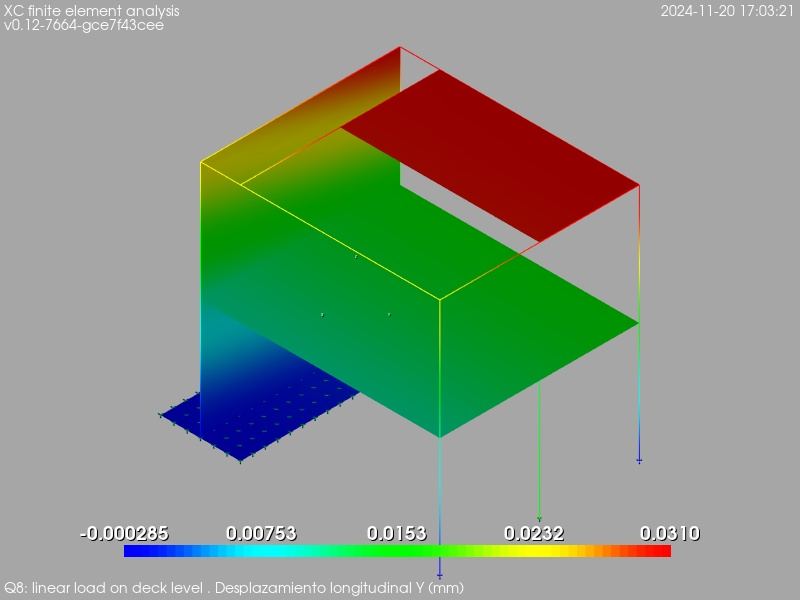
\includegraphics[width=\linewidth]{results/graphics/resSimplLC/qlinDeckuY.png}
\caption{Q8: linear load on deck level . Desplazamiento longitudinal Y (mm)}
\label{qlinDeckuY}
\end{center}
\end{figure}
\begin{figure}[ht]
\begin{center}
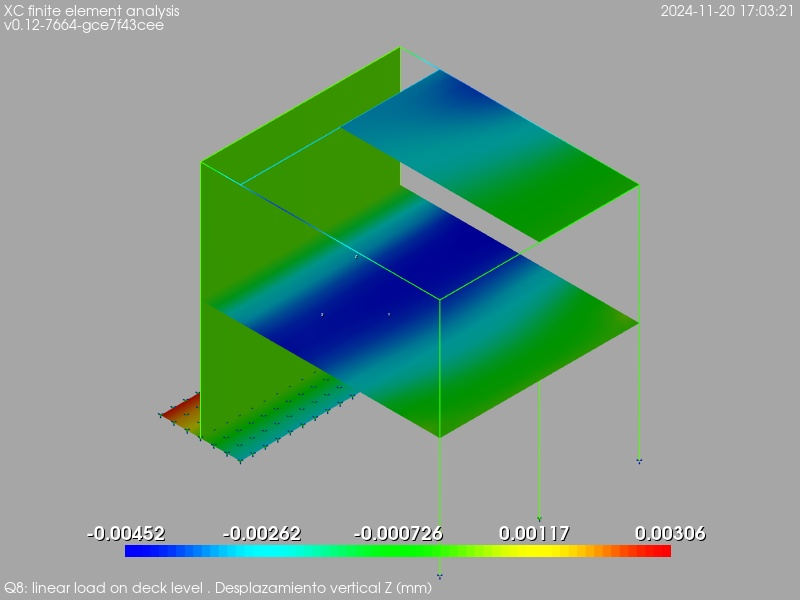
\includegraphics[width=\linewidth]{results/graphics/resSimplLC/qlinDeckuZ.png}
\caption{Q8: linear load on deck level . Desplazamiento vertical Z (mm)}
\label{qlinDeckuZ}
\end{center}
\end{figure}
\begin{figure}[ht]
\begin{center}
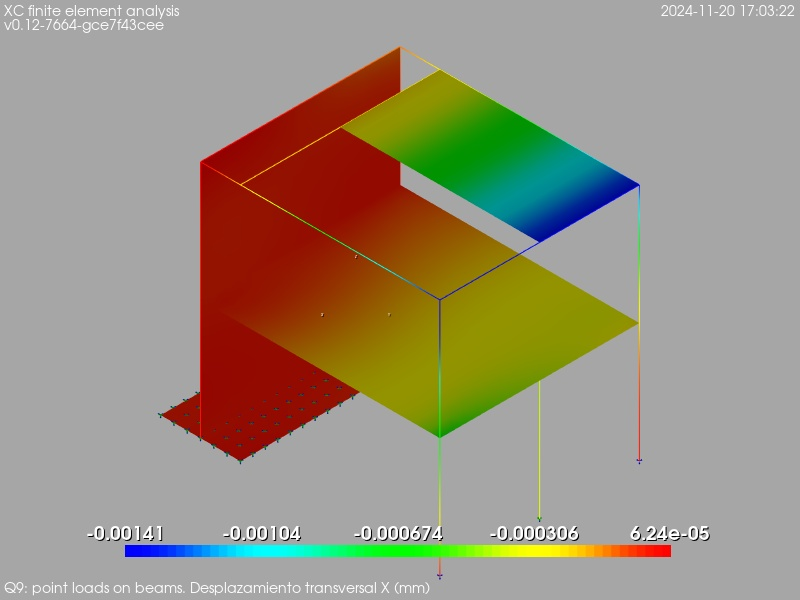
\includegraphics[width=\linewidth]{results/graphics/resSimplLC/QpntBeamsuX.png}
\caption{Q9: point loads on beams. Desplazamiento transversal X (mm)}
\label{QpntBeamsuX}
\end{center}
\end{figure}
\begin{figure}[ht]
\begin{center}
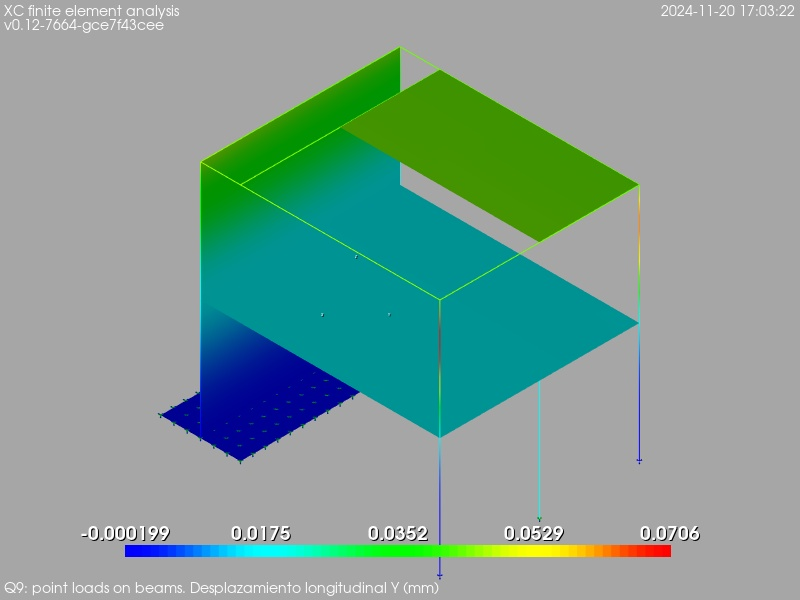
\includegraphics[width=\linewidth]{results/graphics/resSimplLC/QpntBeamsuY.png}
\caption{Q9: point loads on beams. Desplazamiento longitudinal Y (mm)}
\label{QpntBeamsuY}
\end{center}
\end{figure}
\begin{figure}[ht]
\begin{center}
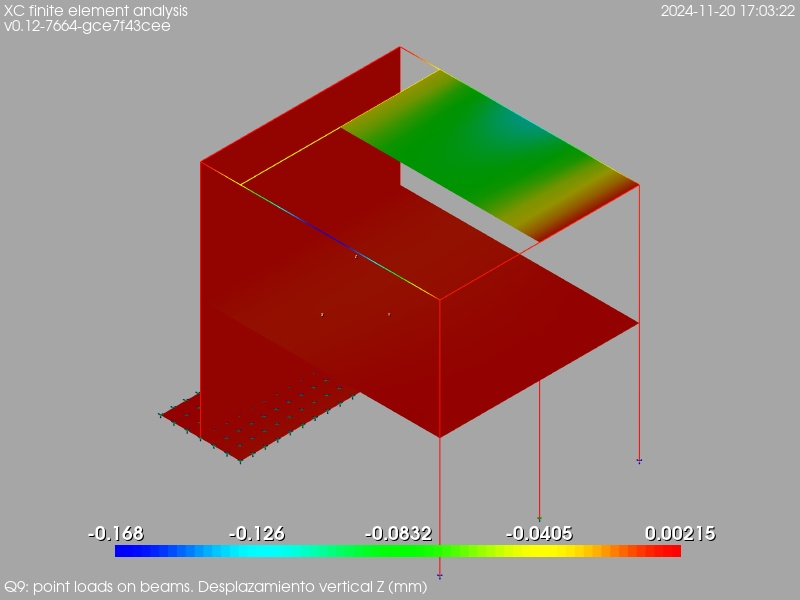
\includegraphics[width=\linewidth]{results/graphics/resSimplLC/QpntBeamsuZ.png}
\caption{Q9: point loads on beams. Desplazamiento vertical Z (mm)}
\label{QpntBeamsuZ}
\end{center}
\end{figure}
\begin{figure}[ht]
\begin{center}
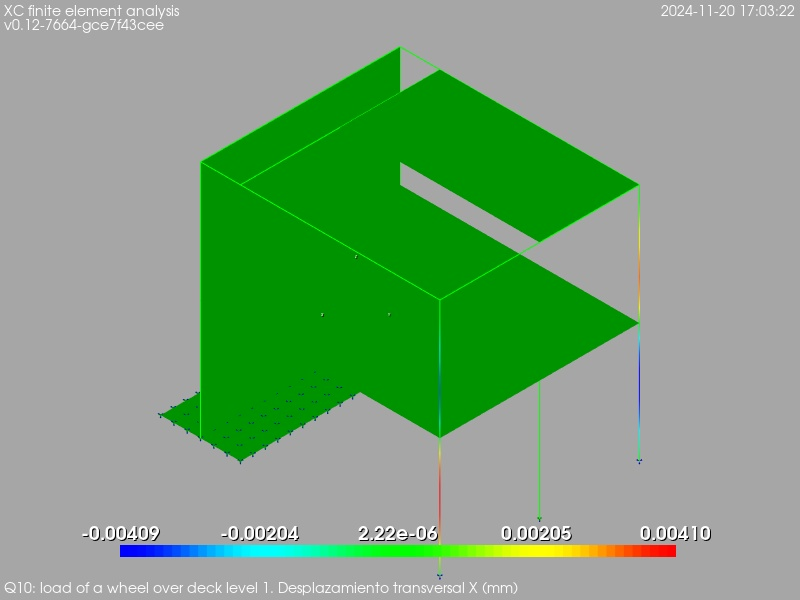
\includegraphics[width=\linewidth]{results/graphics/resSimplLC/QwheelDeck1uX.png}
\caption{Q10: load of a wheel over deck level 1. Desplazamiento transversal X (mm)}
\label{QwheelDeck1uX}
\end{center}
\end{figure}
\begin{figure}[ht]
\begin{center}
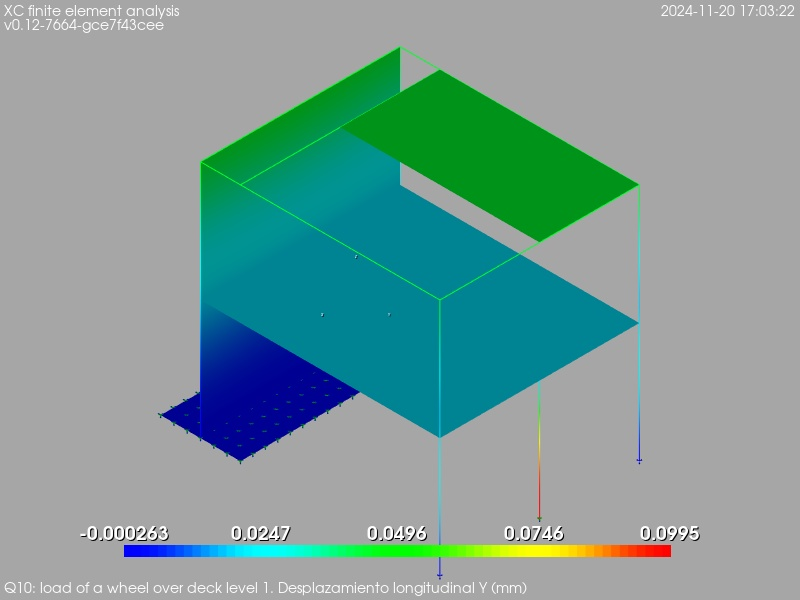
\includegraphics[width=\linewidth]{results/graphics/resSimplLC/QwheelDeck1uY.png}
\caption{Q10: load of a wheel over deck level 1. Desplazamiento longitudinal Y (mm)}
\label{QwheelDeck1uY}
\end{center}
\end{figure}
\begin{figure}[ht]
\begin{center}
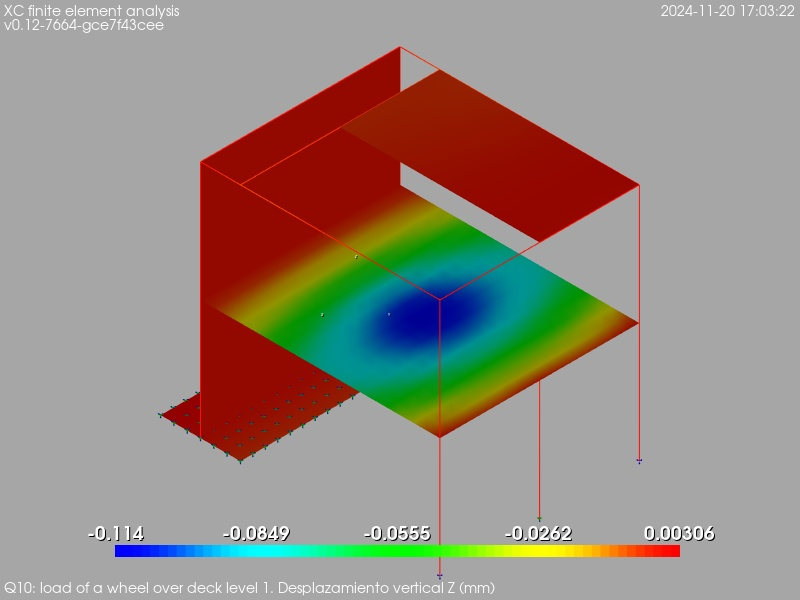
\includegraphics[width=\linewidth]{results/graphics/resSimplLC/QwheelDeck1uZ.png}
\caption{Q10: load of a wheel over deck level 1. Desplazamiento vertical Z (mm)}
\label{QwheelDeck1uZ}
\end{center}
\end{figure}
\begin{figure}[ht]
\begin{center}
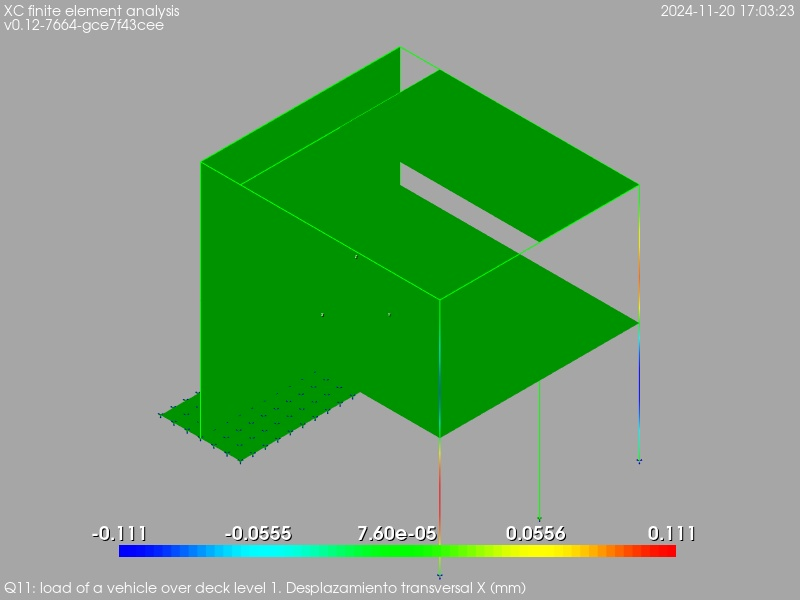
\includegraphics[width=\linewidth]{results/graphics/resSimplLC/QvehicleDeck1uX.png}
\caption{Q11: load of a vehicle over deck level 1. Desplazamiento transversal X (mm)}
\label{QvehicleDeck1uX}
\end{center}
\end{figure}
\begin{figure}[ht]
\begin{center}
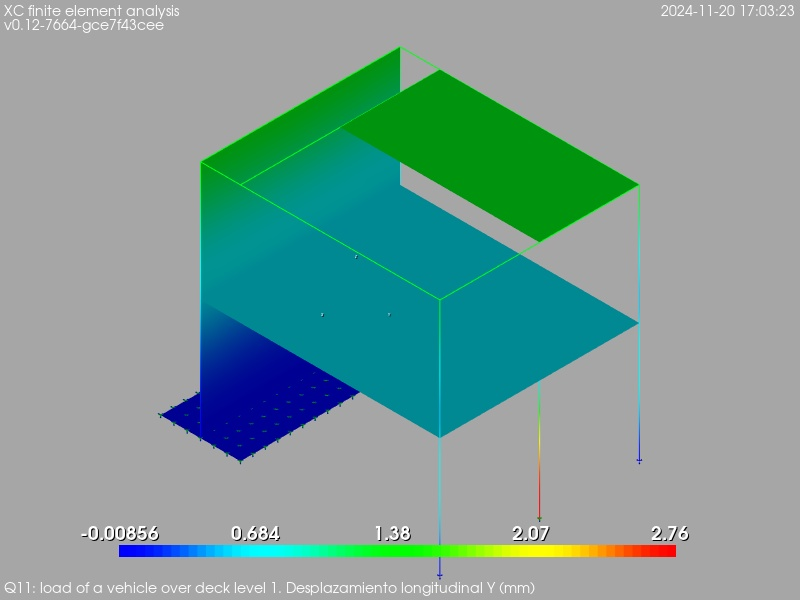
\includegraphics[width=\linewidth]{results/graphics/resSimplLC/QvehicleDeck1uY.png}
\caption{Q11: load of a vehicle over deck level 1. Desplazamiento longitudinal Y (mm)}
\label{QvehicleDeck1uY}
\end{center}
\end{figure}
\begin{figure}[ht]
\begin{center}
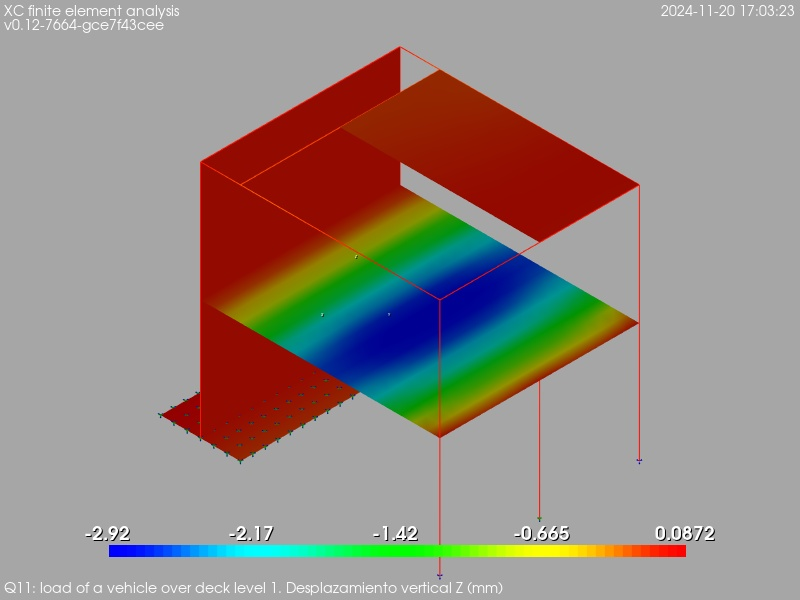
\includegraphics[width=\linewidth]{results/graphics/resSimplLC/QvehicleDeck1uZ.png}
\caption{Q11: load of a vehicle over deck level 1. Desplazamiento vertical Z (mm)}
\label{QvehicleDeck1uZ}
\end{center}
\end{figure}
\begin{figure}[ht]
\begin{center}
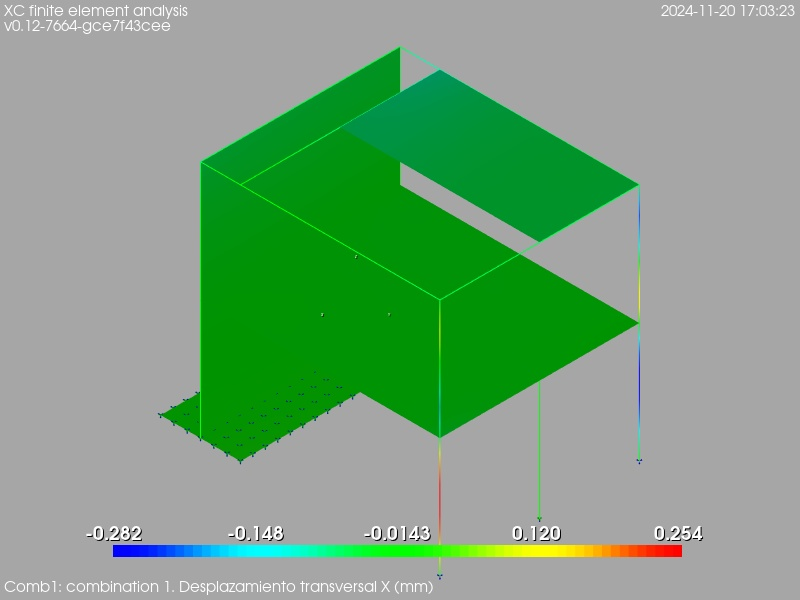
\includegraphics[width=\linewidth]{results/graphics/resSimplLC/LS1uX.png}
\caption{Comb1: combination 1. Desplazamiento transversal X (mm)}
\label{LS1uX}
\end{center}
\end{figure}
\begin{figure}[ht]
\begin{center}
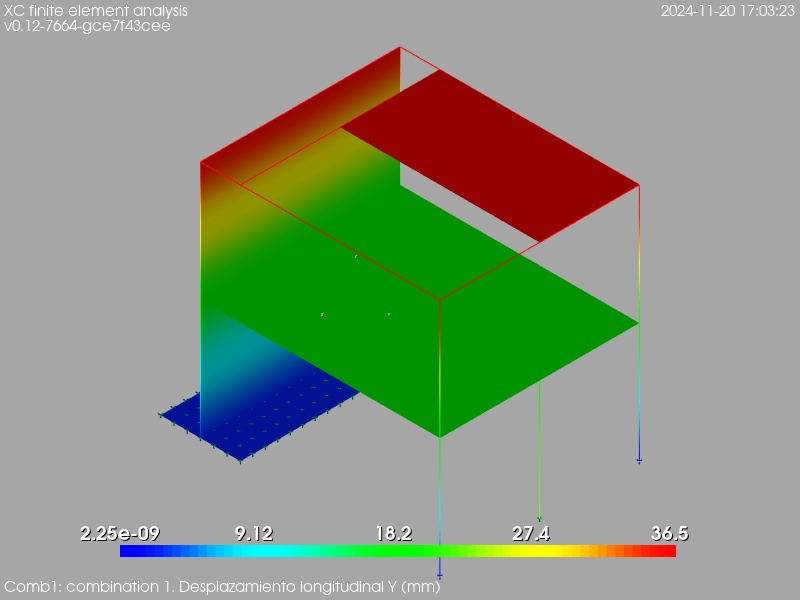
\includegraphics[width=\linewidth]{results/graphics/resSimplLC/LS1uY.png}
\caption{Comb1: combination 1. Desplazamiento longitudinal Y (mm)}
\label{LS1uY}
\end{center}
\end{figure}
\begin{figure}[ht]
\begin{center}
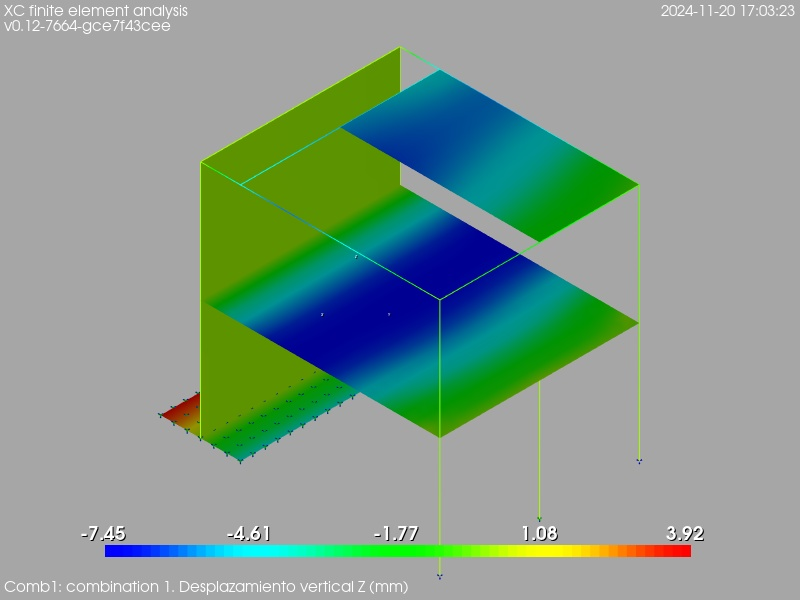
\includegraphics[width=\linewidth]{results/graphics/resSimplLC/LS1uZ.png}
\caption{Comb1: combination 1. Desplazamiento vertical Z (mm)}
\label{LS1uZ}
\end{center}
\end{figure}
\begin{figure}[ht]
\begin{center}
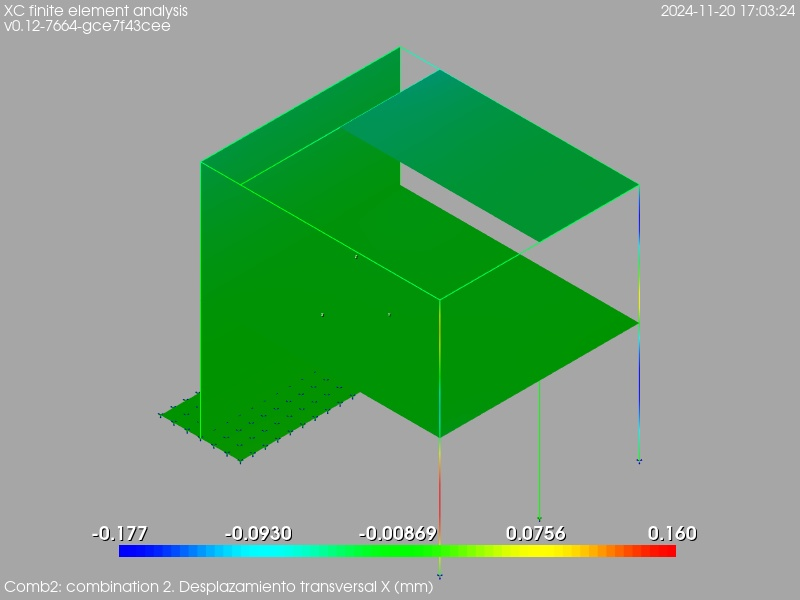
\includegraphics[width=\linewidth]{results/graphics/resSimplLC/LS2uX.png}
\caption{Comb2: combination 2. Desplazamiento transversal X (mm)}
\label{LS2uX}
\end{center}
\end{figure}
\begin{figure}[ht]
\begin{center}
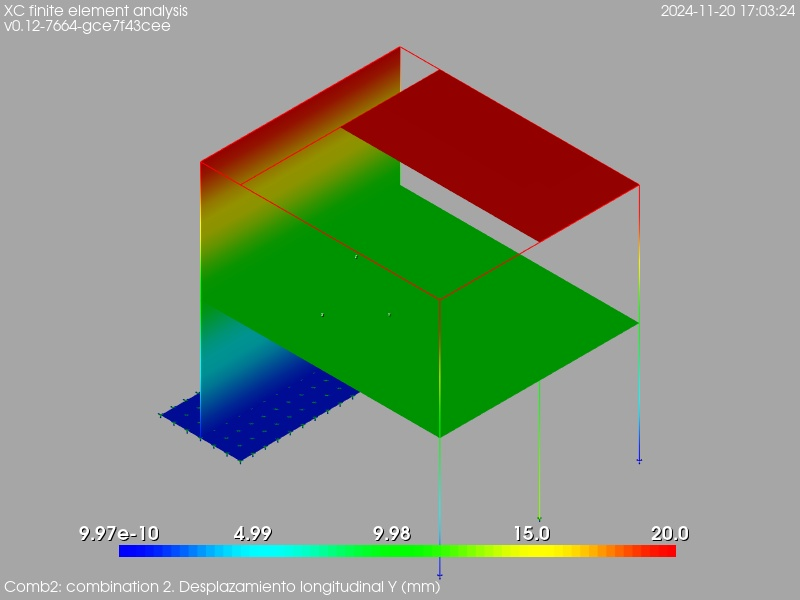
\includegraphics[width=\linewidth]{results/graphics/resSimplLC/LS2uY.png}
\caption{Comb2: combination 2. Desplazamiento longitudinal Y (mm)}
\label{LS2uY}
\end{center}
\end{figure}
\begin{figure}[ht]
\begin{center}
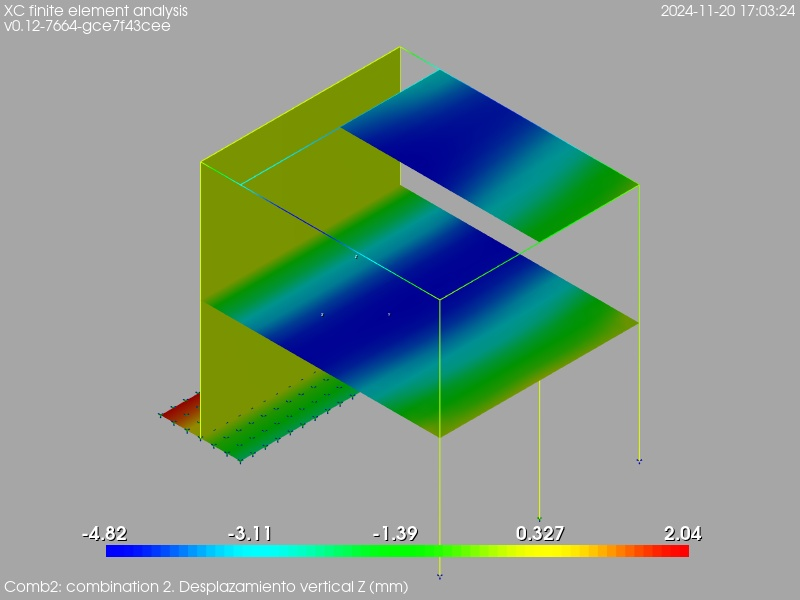
\includegraphics[width=\linewidth]{results/graphics/resSimplLC/LS2uZ.png}
\caption{Comb2: combination 2. Desplazamiento vertical Z (mm)}
\label{LS2uZ}
\end{center}
\end{figure}
\clearpage 
